\chapter{DatasetAnalyzer: implementación y visualizaciones descriptivas}
\label{appendix:visualizaciones_datasetanalyzer}

Este apéndice documenta, en conjunto, los aspectos de implementación de la clase \textit{DatasetAnalyzer} referenciados en la Sección~\ref{sec:caracterizacion_datasets} del Capítulo~\ref{cap:caracterizacion_datasets}, y las visualizaciones descriptivas que dicha clase generó tanto sobre los datos originales (\textit{raw}) como sobre las cohortes curadas de los dominios de mama y colorrectal.

\section{Detalles de implementación de DatasetAnalyzer}
\label{appendix:detalles_datasetanalyzer}

\subsection{Reglas de tipificación de variables}

La tipificación de variables del \textit{DatasetAnalyzer} se basó en reglas declarativas para variables conocidas (por ejemplo, edad tratada como numérica, sexo o diagnóstico como categóricos, y campos de fecha como variables temporales) y en un mecanismo de detección automática para el resto de las columnas. Este mecanismo automático utilizó proporciones de conversión numérica y temporal sobre los valores observados en cada columna, es decir, la fracción de valores que podían convertirse exitosamente a tipo numérico o a tipo fecha, además de la cardinalidad observada (número de categorías distintas) para distinguir entre variables categóricas, booleanas y de texto libre. Cuando la proporción de conversión numérica o temporal superaba un umbral predefinido, la columna se tipificaba en consecuencia; en caso contrario, se evaluaba la cardinalidad relativa al número de registros para decidir entre una codificación categórica (baja cardinalidad) o de texto libre (alta cardinalidad, valores mayoritariamente únicos).

\subsection{Procesamiento semántico de metadatos textuales en HISTAI}

Dado que gran parte de los metadatos clínicos de HISTAI se encontraba en campos de texto libre, especialmente en descripciones diagnósticas con abreviaturas, sinonimia y distintos niveles de especificidad clínica, no resultaba adecuado generar visualizaciones directas sobre este texto heterogéneo. Por ello, se incorporó una etapa intermedia de estructuración semántica, aplicada específicamente sobre las subcohortes HISTAI-Breast, HISTAI-CRC-B1 e HISTAI-CRC-B2, mediante \textit{scripts} de mapeo orientados a transformar los campos diagnósticos originales en variables derivadas.

En HISTAI-Breast, el procedimiento permitió normalizar variantes diagnósticas e identificar lateralidad anatómica, generando variables derivadas como diagnóstico normalizado, grupo taxonómico, subgrupo taxonómico, lateralidad y estado de revisión diagnóstica. En HISTAI-CRC-B1 y HISTAI-CRC-B2, además de la normalización textual, se incorporó la detección del sitio anatómico y la agrupación de diagnósticos en categorías amplias: lesiones inflamatorias o no neoplásicas, precursores benignos, neoplasias malignas, categorías inespecíficas y casos sospechosos. Esta etapa permitió transformar texto clínico heterogéneo en una representación más estable y comparable, sin modificar la información de base reportada por el \textit{dataset}.

\section{Visualizaciones descriptivas originales}
\label{sec:app_c_visualizaciones_originales}

En esta sección se presentan las visualizaciones descriptivas generadas automáticamente a partir de los metadatos tabulares de cada conjunto de datos analizado mediante la clase \textit{DatasetAnalyzer}, sobre los datos \textit{raw} previos a cualquier transformación.

El conjunto completo de figuras (numéricas y categóricas) para los doce recursos procesados está disponible en el siguiente enlace de Google Drive:

\medskip
\centerline{\url{https://drive.google.com/drive/folders/1KefjTu5jXc06eKCe9i1kOdYnaUsgZvvu?usp=sharing}}
\medskip

La estructura de la carpeta sigue la nomenclatura de cada dataset, con subcarpetas \texttt{plots\_numeric} y \texttt{plots\_categorical} que contienen, respectivamente, histogramas con \textit{boxplots} para variables numéricas y gráficos de barras para variables categóricas.

La Tabla~\ref{tab:appc_datasets_resumen} resume los datasets incluidos y la cantidad de figuras generadas para cada uno.

\begin{table}[htbp]
\centering
\caption{Resumen de visualizaciones generadas por dataset.}
\label{tab:appc_datasets_resumen}
\small
\begin{tabular}{lrr}
\toprule
Dataset & Numéricas & Categóricas \\
\midrule
Ovarian Bevacizumab Response & 3 & 6 \\
BCNB & 3 & 10 \\
CLWD & 1 & 9 \\
NDB-UFES & 1 & 12 \\
TDBTA & 3 & 8 \\
SurGen-SR386 & 1 & 25 \\
SurGen-SR1482 & 1 & 11 \\
HSI-BC (HSIBRCA) & -- & -- \\
SOPHIE & 1 & 8 \\
HISTAI-Breast & 1 & 11 \\
HISTAI-CRC-B1 & 1 & 12 \\
HISTAI-CRC-B2 & 1 & 12 \\
\bottomrule
\end{tabular}
\end{table}

A modo ilustrativo, la Figura~\ref{fig:bcnb-age} muestra la distribución de edad en BCNB tal como fue registrada originalmente, y la Figura~\ref{fig:bcnb-molecular-subtype} presenta los subtipos moleculares en el mismo conjunto. Estas distribuciones corresponden a los datos sin curar y se incluyen aquí como referencia de la línea base previa al proceso de armonización descrito en la Sección~\ref{sec:caracterizacion_datasets}.

\begin{figure}[htbp]
\centering
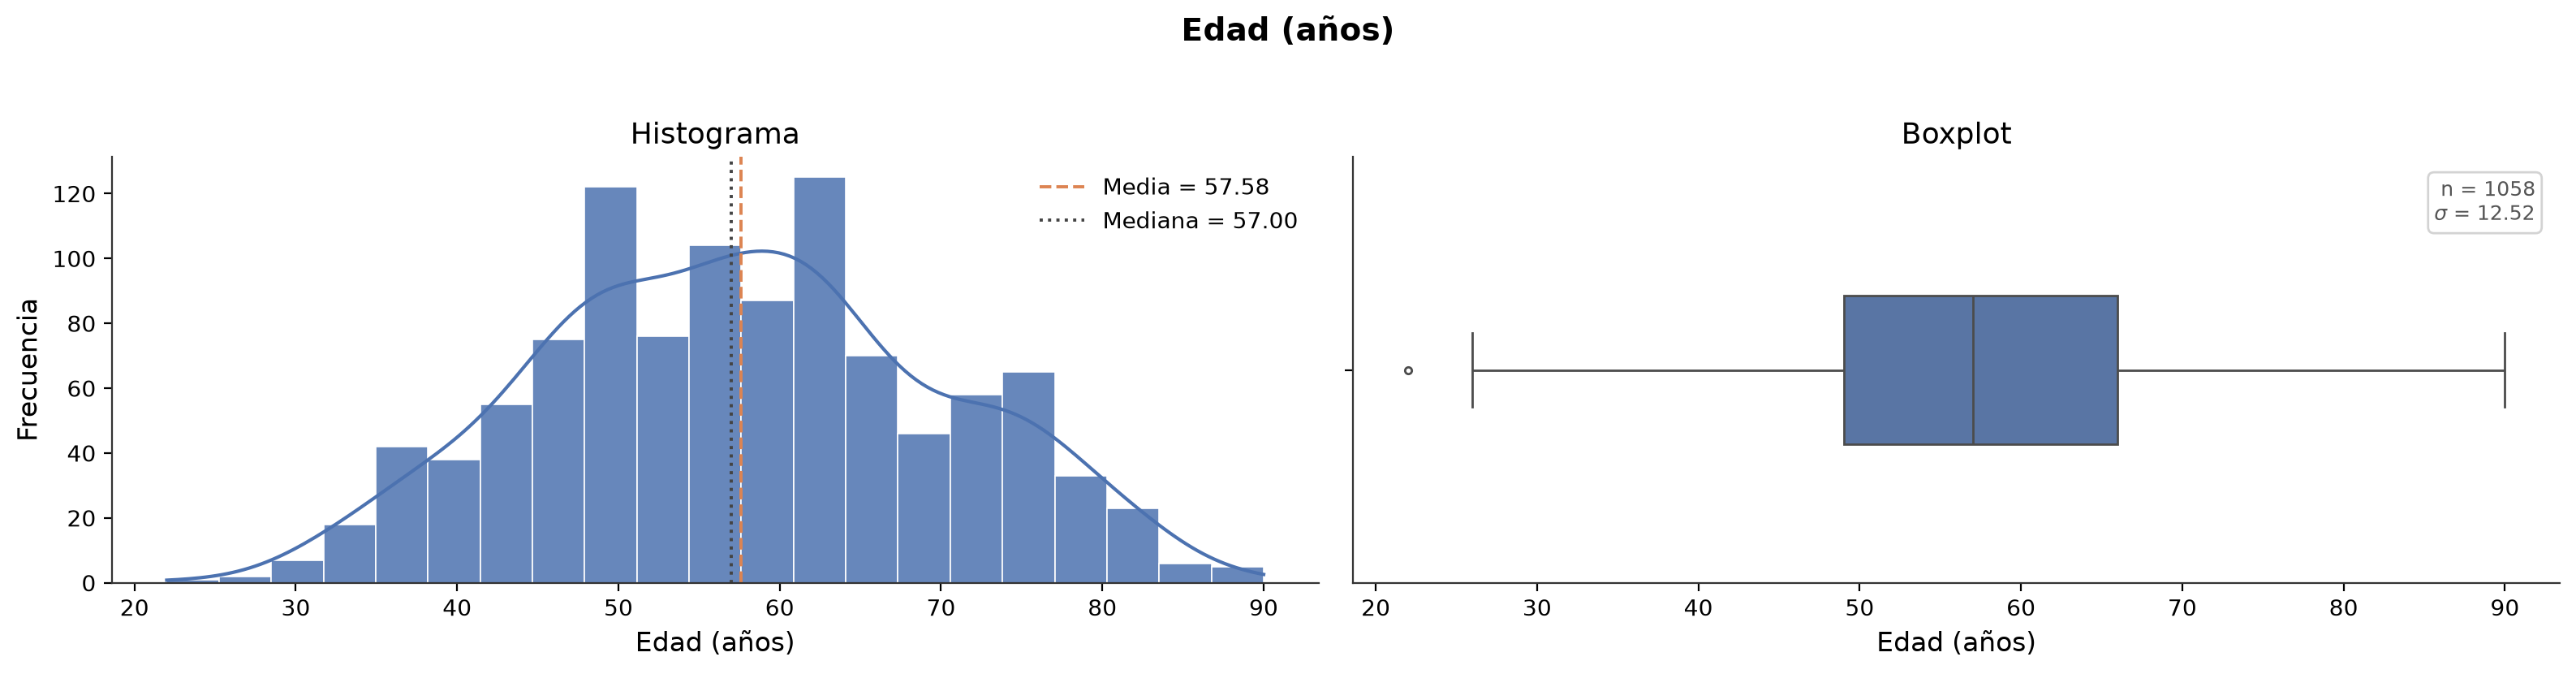
\includegraphics[width=0.75\textwidth]{images/fig41-bcnb-age.png}
\caption{Distribución de la variable \textit{Age} en BCNB (datos originales).}
\label{fig:bcnb-age}
\end{figure}

\begin{figure}[htbp]
\centering
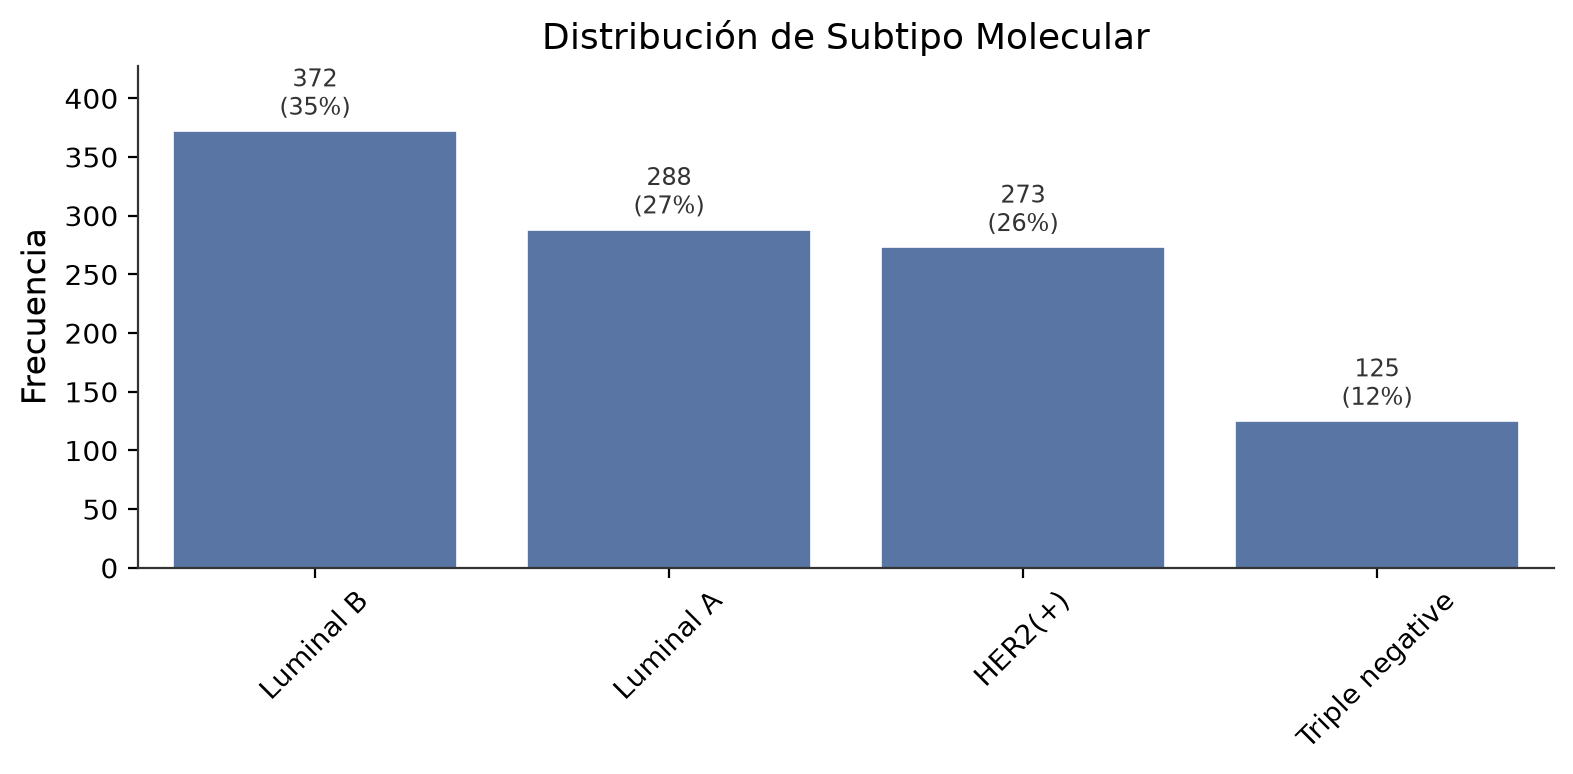
\includegraphics[width=0.75\textwidth]{images/fig43-bcnb-molecular-subtype.png}
\caption{Distribución de la variable \textit{Molecular subtype} en BCNB (datos originales).}
\label{fig:bcnb-molecular-subtype}
\end{figure}

% \section{Visualizaciones post-curación}
% \label{appendix:visualizaciones_postcuracion}

% Esta sección presenta las visualizaciones de las distribuciones post-curación referenciadas en la Sección~\ref{sec:visualizacion_distribuciones} del Capítulo~\ref{cap:caracterizacion_datasets}. Las Figuras~\ref{fig:surgen-site-total-curated}~y~\ref{fig:surgen-side-total-curated} presentan la distribución agregada del sitio tumoral y la lateralidad en SurGen (SR386 y SR1482 combinados), tras el proceso de armonización descrito en la Sección~\ref{sec:caracterizacion_datasets}.

% \begin{figure}[htbp]
% \centering
% 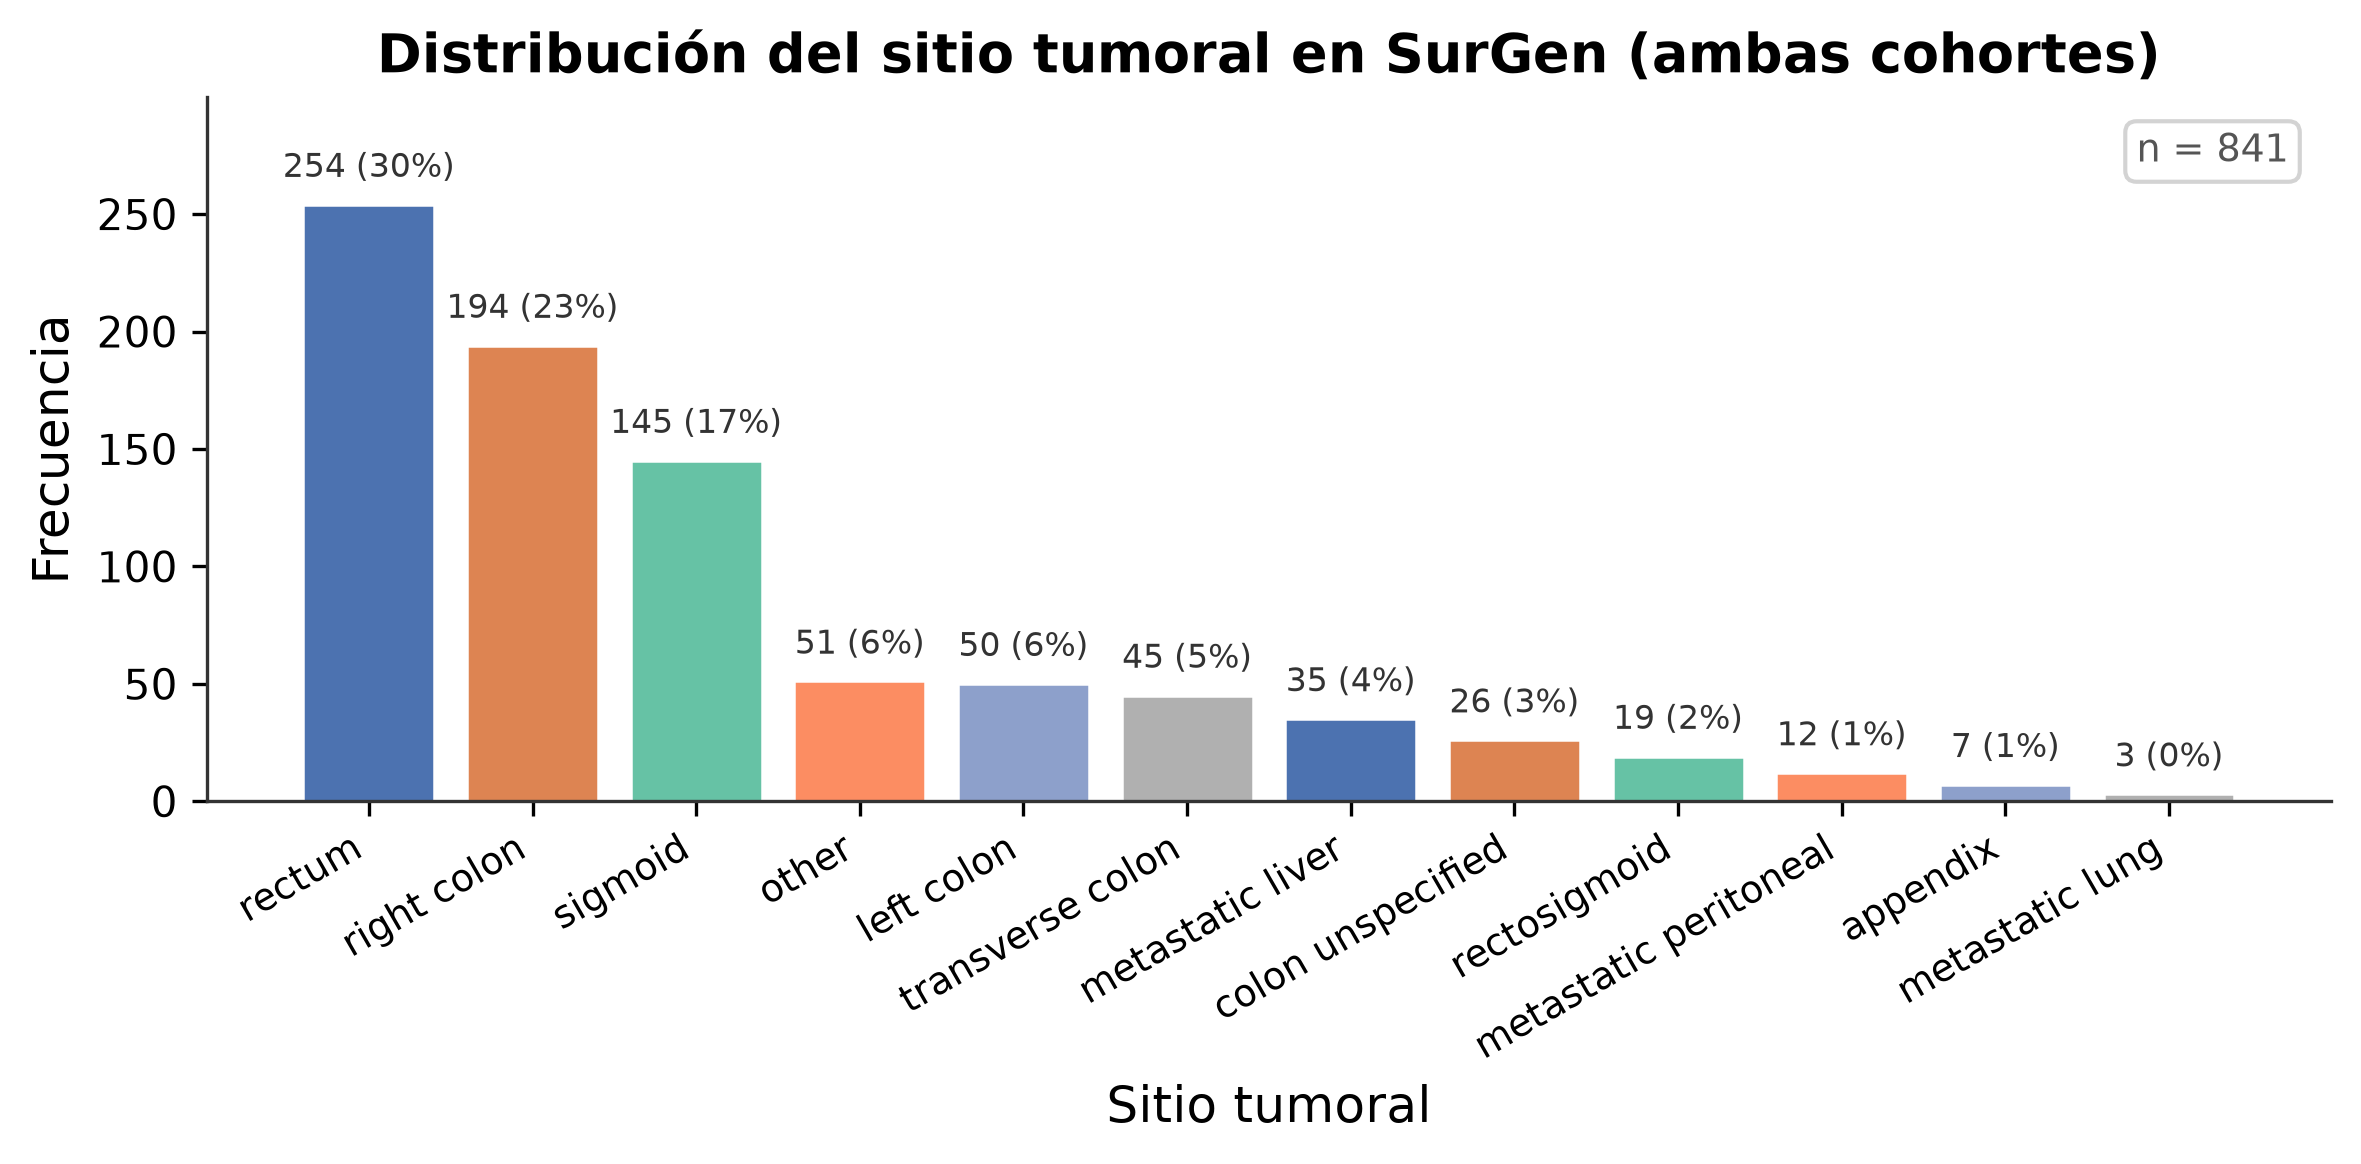
\includegraphics[width=0.8\textwidth]{images/fig47-surgen-site-total-curated.png}
% \caption{Distribución agregada del sitio tumoral en SurGen (SR386~+~SR1482 combinados, post-curación).}
% \label{fig:surgen-site-total-curated}
% \end{figure}

% \begin{figure}[htbp]
% \centering
% 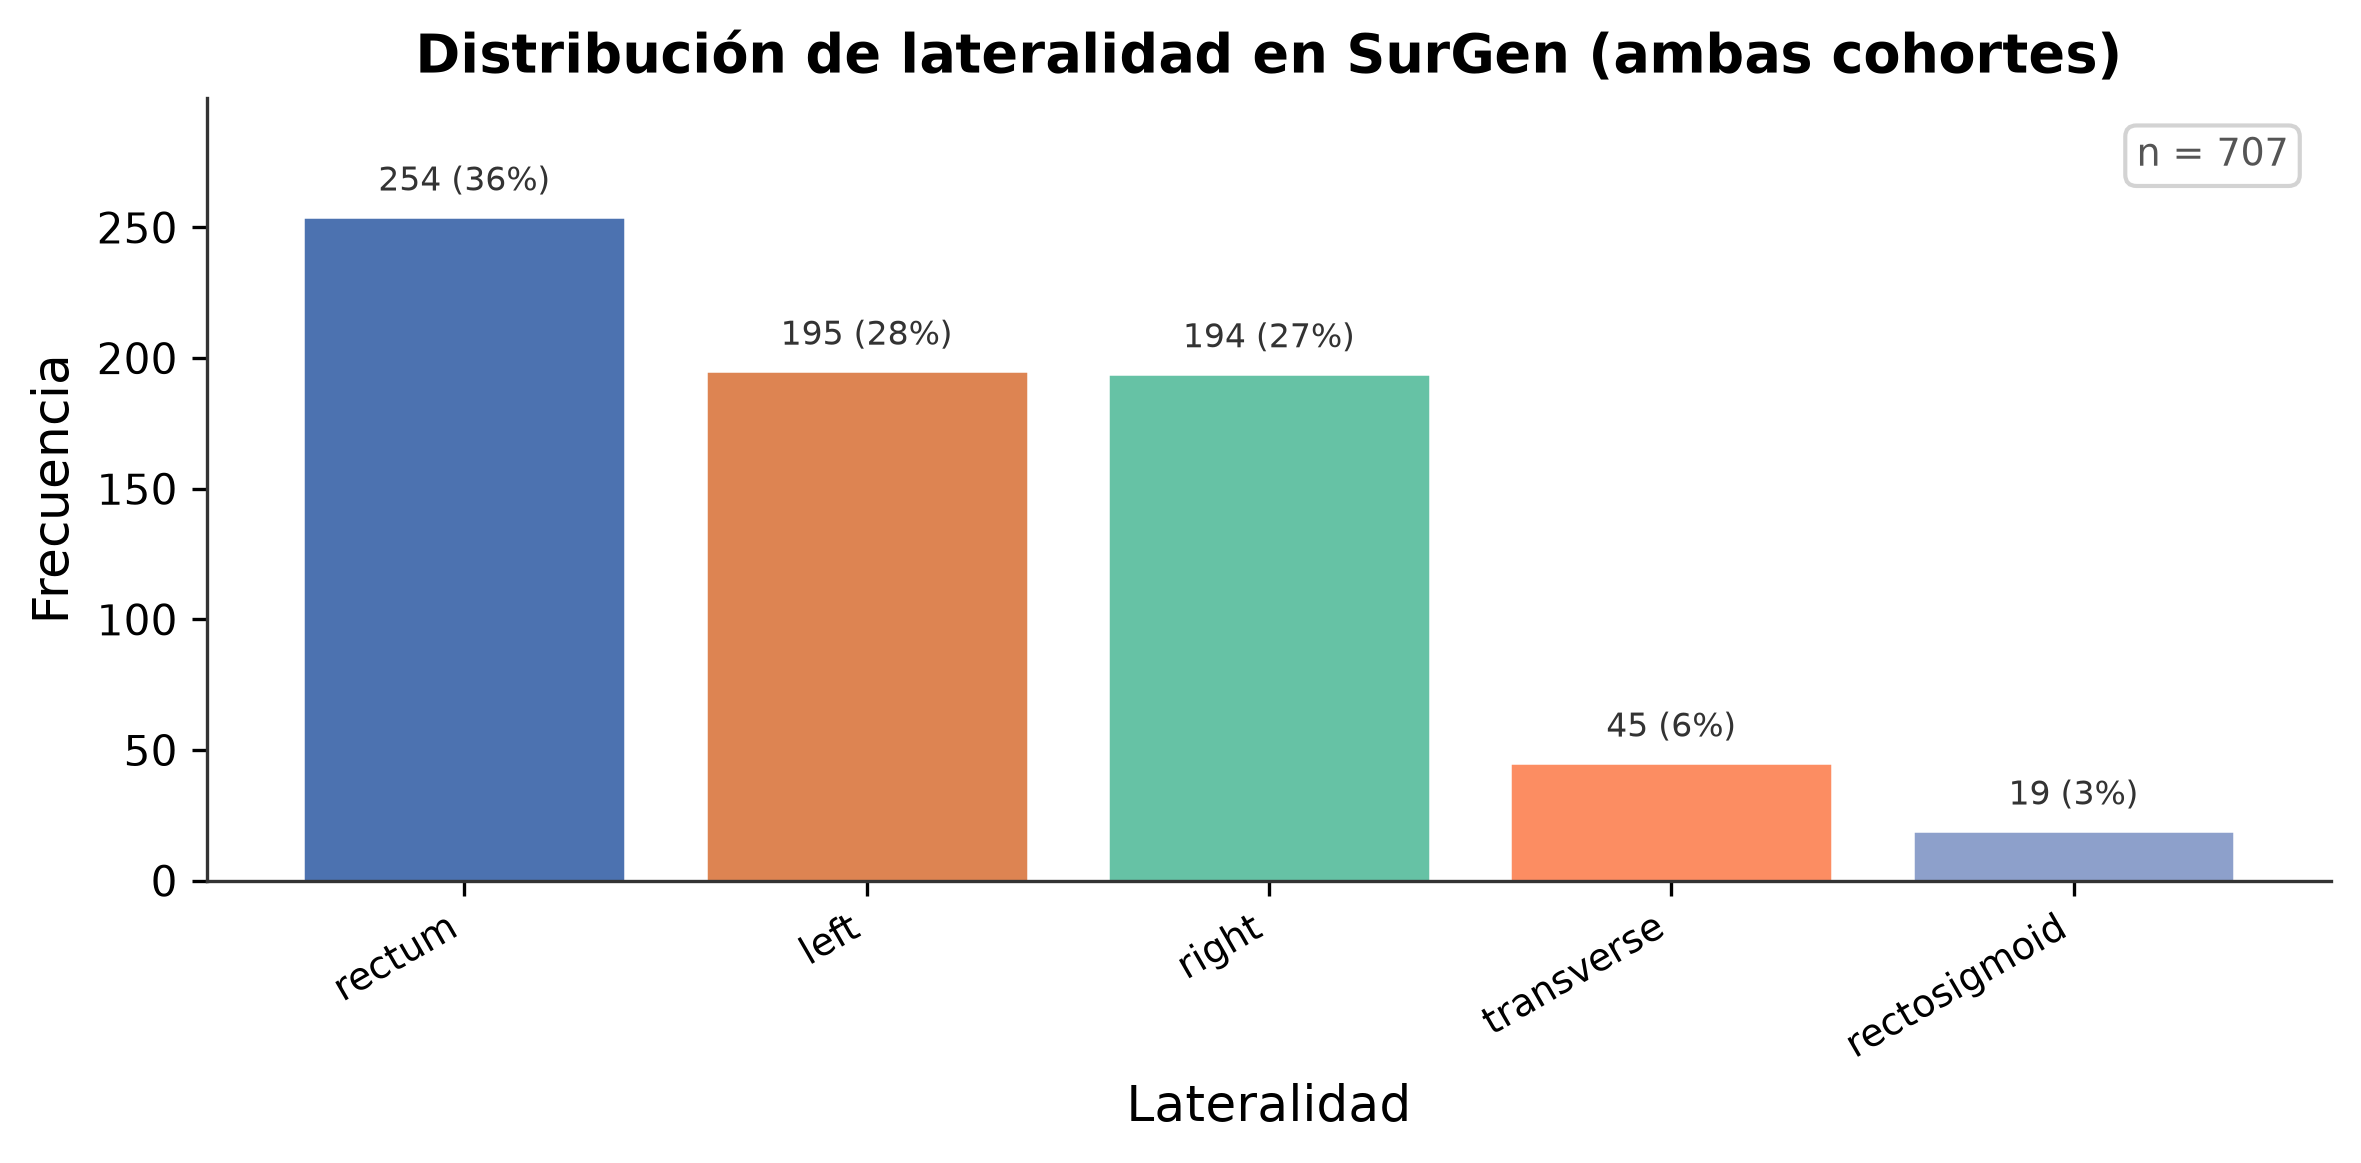
\includegraphics[width=0.8\textwidth]{images/fig48-surgen-side-total-curated.png}
% \caption{Distribución agregada de lateralidad en SurGen (SR386~+~SR1482 combinados, post-curación). La lateralidad se deriva del sitio tumoral y permite una comparación más compacta entre cohortes.}
% \label{fig:surgen-side-total-curated}
% \end{figure}


\section{Extracción de variables clínicas desde texto libre en HISTAI}
\label{appendix:extraccion_histai}

Los metadatos clínicos de HISTAI se encuentran mayormente en campos de texto libre dentro del informe histopatológico. Para recuperar variables comparables con los demás conjuntos de datos, se implementó un pipeline de extracción basado en expresiones regulares y recodificación explícita, ejecutado sobre un campo de texto unificado por caso. Esta sección documenta las fuentes textuales utilizadas, los patrones aplicados por variable, los criterios de resolución de conflictos, el tratamiento de los casos no parseables, la cobertura resultante y las limitaciones del proceso, incluyendo la ausencia de una validación manual con muestra independiente.

\subsection{Fuentes textuales y composición del texto analizado}

Para cada subcohorte se concatenaron los campos narrativos disponibles en el orden indicado (Tabla~\ref{tab:anexo_campos_histai}), generando el campo \texttt{full\_text} sobre el cual se ejecutaron todas las reglas. El orden de concatenación es relevante porque, salvo indicación contraria, las reglas recuperan la \emph{primera} coincidencia en el texto resultante: los campos que aparecen primero adquieren prioridad de facto.

\begin{table}[htbp]
\centering
\caption{Campos narrativos considerados en la extracción por subcohorte HISTAI.}
\label{tab:anexo_campos_histai}
\small
\begin{tabular}{lccl}
\toprule
Subcohorte & N & Campos concatenados (en orden) \\
\midrule
HISTAI-Breast & 1489 & diagnosis, conclusion, additional\_info, micro\_protocol  \\
HISTAI-CRC-B1 & 878 & diagnosis, conclusion, grossing, micro\_protocol, additional\_info  \\
HISTAI-CRC-B2 & 57 & diagnosis, conclusion, grossing, micro\_protocol, additional\_info  \\
\bottomrule
\end{tabular}
\end{table}

Además, la etapa de mapeo semántico previa (descrita en la Sección~\ref{appendix:detalles_datasetanalyzer}) generó, a partir del campo \texttt{diagnosis}, las variables derivadas de diagnóstico (grupo taxonómico y sitio/lateralidad taxonómicos), que sirven de base para la clasificación de sitio y lateralidad del dominio colorrectal.

\subsection{Reglas de extracción en el dominio de mama}

La Tabla~\ref{tab:anexo_reglas_mama} resume los patrones aplicados sobre \texttt{full\_text} en HISTAI-Breast y su recodificación. Las menciones se realizan sobre texto en minúsculas; en ER/PR la búsqueda está acotada a la oración (el patrón considera texto hasta el primer punto), mientras en HER2 y Ki-67 la búsqueda es global al documento.

\begin{table}[htbp]
\centering
\caption{Reglas de extracción por biomarcador en HISTAI-Breast.}
\label{tab:anexo_reglas_mama}
\footnotesize
\setlength{\tabcolsep}{3pt}
\resizebox{\textwidth}{!}{%
\begin{tabular}{p{1.6cm}p{4.6cm}p{6.2cm}p{3.4cm}}
\toprule
Variable & Patrón aplicado & Lectura y recodificación & Ejemplo (abreviado) \\
\midrule
ER & \texttt{\textbackslash{}ber\textbackslash{}b[.\^{}]*negative} primero; si no, \texttt{\textbackslash{}ber\textbackslash{}b[.\^{}]*positive} & \emph{negative} $\rightarrow$ 0 (negativo); \emph{positive} $\rightarrow$ 1 (positivo); si ninguno en la oración, sin dato & ``\ldots ER: positive (more than 10\% of tumor cells) \ldots'' $\rightarrow$ 1 \\
PR & \texttt{\textbackslash{}bpr\textbackslash{}b[.\^{}]*negative} primero; si no, \texttt{\textbackslash{}bpr\textbackslash{}b[.\^{}]*positive} & idem ER & ``\ldots PR: positive \ldots'' $\rightarrow$ 1 \\
HER2 & \texttt{her2[.\^{}0-9]*([0-3])\textbackslash{}s*+?} & score 0 o 1 $\rightarrow$ 0 (negativo/bajo); 2 $\rightarrow$ 1 (equívoco); 3 $\rightarrow$ 2 (positivo) & ``\ldots anti-Her2 (c-erbB-2) antibody --- 3 points: strong complete membrane staining \ldots'' $\rightarrow$ 2 \\
HER2 (fallback) & si sin score: \texttt{her2} y \texttt{negative} en el documento; luego \texttt{her2} y (\texttt{undetermined} o \texttt{equivocal}) & \emph{negative} $\rightarrow$ 0; \emph{undetermined}/\emph{equivocal} $\rightarrow$ 1 (equívoco) & ``\ldots HER2 status undetermined \ldots'' $\rightarrow$ 1 \\
Ki-67 & \texttt{ki-?67[.\^{}0-9]*([0-9]+(?:\textbackslash{}.[0-9]+)?)} & primer número tras la mención; categorías: $<10$ baja, $10$--$20$ intermedia, $>20$ alta & ``\ldots Ki-67 proliferation index: 30\% \ldots'' $\rightarrow$ 30 (alta) \\
Subtipo & menciones directas en el orden: \texttt{triple negative}; \texttt{luminal a}; \texttt{luminal b}; \texttt{her2} + (\texttt{positive} o \texttt{3+}) & Triple negative; Luminal A; Luminal B; HER2+; sin derivación desde biomarcadores & ``\ldots Surrogate molecular subtype: Luminal A \ldots'' $\rightarrow$ Luminal A \\
\bottomrule
\end{tabular}%
}
\end{table}

Nota: la codificación de subtipo se basa exclusivamente en la mención explícita del subtipo en el informe; no se deriva de los biomarcadores extraídos. Como referencia de armonización, en BCNB los valores estructurados se recodificaron con la misma escala (ER/PR binarios; HER2 0/0+ y 1/1+ $\rightarrow$ 0, 2/2+ $\rightarrow$ 1, 3/3+ $\rightarrow$ 2; Ki-67 con rango promediado: \texttt{"15-20"} $\rightarrow$ 15) y en HSI-BC los códigos \texttt{0/1/2} se interpretaron como negativo/positivo/equívoco (HER2) y el código de Ki-67 se convirtió a porcentaje mediante una correspondencia heurística \texttt{\{0,1,2,3,4\}$\rightarrow$\{5,10,20,30,40\}}.

\subsection{Reglas de extracción en el dominio colorrectal}

\paragraph{Sitio anatómico.} La detección se realiza en dos pasos. Primero, sobre el diagnóstico normalizado (con expansión de códigos ICD-10 como C18.\textit{x}, C19, C20, D12.5 y D37.7), se aplica una lista ordenada de 11 reglas de sitio (rectosigmoide, recto, sigmoide, colon descendente, flexura esplénica, colon transverso, flexura hepática, colon ascendente, ciego, canal anal y colon inespecífico), devolviendo el primer patrón que coincide; si ninguno, la etiqueta \texttt{unspecified}. Segundo, las etiquetas resultantes se agrupan en el vocabulario de tarea de nueve clases que comparten HISTAI-CRC-B1, HISTAI-CRC-B2 y SurGen:

\begin{center}
\small
\texttt{\{rectum, sigmoid, right\_colon, left\_colon, transverse\_colon, rectosigmoid, colon\_unspecified, metastatic\_liver, other\}}
\end{center}

La categoría \emph{Otros} (\texttt{other}) queda definida por la regla de caída (sin coincidencia de ningún patrón). En HISTAI-CRC-B1 su composición observada es: diagnósticos sin mención de sitio (117 casos), flexura esplénica (11) y canal anal (2); en SurGen, la clase colapsa además las localizaciones de baja frecuencia declaradas en la Sección~\ref{sec:caracterizacion_datasets} (apéndice, metástasis peritoneales y pulmonares; n=12, 7 y 3, respectivamente). Cabe señalar una limitación del mapeo: al aplicarse sobre la etiqueta taxonómica normalizada (con guiones bajos) y no sobre el texto original, el literal \texttt{hepatic flexure} (con espacio) no activa la regla de colon derecho, y la subcadena \texttt{hepatic} activa la regla de metástasis hepática; por ello, 18 casos de flexura hepática del colon (C18.3) quedaron codificados como \texttt{metastatic\_liver} en HISTAI-CRC-B1. El impacto de esta decisión se limita a la composición de la clase \texttt{metastatic\_liver} (en la Tabla~\ref{tab:resumen_frecuencias_colorrectal}, 18 casos, 2,1\,\%).

\paragraph{Lateralidad.} Derivada del sitio agrupado: colon derecho $\rightarrow$ \texttt{right}; colon izquierdo y sigmoide $\rightarrow$ \texttt{left}; transverso $\rightarrow$ \texttt{transverse}; recto $\rightarrow$ \texttt{rectum}; rectosigmoide $\rightarrow$ \texttt{rectosigmoid}; el resto (colon inespecífico, \emph{Otros} y metástasis hepática) queda sin dato.

\paragraph{Estadificación y variables histopatológicas.} Sobre \texttt{full\_text} se extraen, con el mismo criterio de primera coincidencia: grado (G1--G3 por \texttt{g1}/\texttt{grade: 1}/\texttt{1-high grade differentiation} y equivalentes verbales \emph{well/moderately/poorly differentiated}); etapa patológica por patrones \texttt{pt([0-4][ab]?)}, \texttt{pn([0-2][abc]?)} y \texttt{pm([01][abcx]?)} (con variante clínica \texttt{cm1} $\rightarrow$ cM1); ganglios examinados y positivos mediante \texttt{total number:}, \texttt{number examined:}, \texttt{number of involved/affected lymph nodes:} y la notación \texttt{n\textit{X}(\textit{p}/\textit{e})}; estado ganglionar derivado del conteo de positivos (0 $\rightarrow$ N0; 1--3 $\rightarrow$ N+(1--3); $>$3 $\rightarrow$ N+(>3); en ausencia de conteo, desde pN); estadio simplificado derivado (M1 $\rightarrow$ IV; N1/N2 $\rightarrow$ III; T3/T4 $\rightarrow$ II; T1/T2 $\rightarrow$ I); e invasión linfovascular y perineural por patrones de presencia/ausencia explícitos. Estas variables se generaron para caracterización descriptiva y comparabilidad con SurGen, pero no fueron seleccionadas como tareas de clasificación en el Capítulo~\ref{cap:seleccion_modelos}. Los biomarcadores moleculares (MMR/MSI, KRAS/NRAS/BRAF) no fueron extraídos desde el texto en las subcohortes HISTAI, quedando como datos faltantes por estructura.

\subsection{Resolución de conflictos}

La política general es \emph{primera coincidencia sobre el texto concatenado}, lo que equivale a priorizar, en mama, \texttt{conclusion} sobre \texttt{additional\_info} sobre \texttt{micro\_protocol}, y en CRC, \texttt{diagnosis} sobre \texttt{conclusion} sobre \texttt{grossing} sobre \texttt{micro\_protocol} sobre \texttt{additional\_info}. Con ello, si un mismo marcador aparece con valores distintos en dos campos (por ejemplo, ``HER2: 2+'' en la conclusión y ``HER2: 3+'' en el protocolo microscópico), prevalece la primera mención. Las excepciones son: (i) ER y PR evalúan la mención negativa antes que la positiva dentro de la oración (ante ambas menciones en la misma oración prevalece \emph{negative}); (ii) en HER2, el score numérico prevalece sobre los fallbacks textuales; y (iii) en subtipo, el orden de evaluación de los patrones (\texttt{triple negative} antes que \texttt{luminal a} antes que \texttt{luminal b} antes que \texttt{her2+}) define la jerarquía.

\subsection{Cobertura resultante}

La Tabla~\ref{tab:anexo_cobertura_mama} reporta la cobertura por marcador en HISTAI-Breast (denominador: cohorte curada, N=1489). La pérdida se concentra en informes sin panel de inmunohistoquímica o sin mención explícita del marcador, no en fallas de parsing de menciones presentes.

\begin{table}[htbp]
\centering
\caption{Cobertura y distribución de clases por marcador en HISTAI-Breast tras la extracción textual.}
\label{tab:anexo_cobertura_mama}
\footnotesize
\setlength{\tabcolsep}{3pt}
\resizebox{\textwidth}{!}{%
\begin{tabular}{lcccl}
\toprule
Marcador & N con dato & Cobertura (\%) & Distribución de clases (n; \%) \\
\midrule
ER & 855 & 57,4 & Negativo 313 (36,6); Positivo 542 (63,4) \\
PR & 849 & 57,0 & Negativo 366 (43,1); Positivo 483 (56,9) \\
HER2 & 878 & 59,0 & Negativo/bajo 133 (15,1); Equívoco 554 (63,1); Positivo 191 (21,8) \\
Ki-67 (numérico) & 889 & 59,7 & Categorías $<10$ / $10$--$20$ / $>20$ \\
Subtipo molecular & 852 & 57,2 & Luminal A 143 (16,8); Luminal B 353 (41,4); HER2+ 281 (33,0); Triple negativo 75 (8,8) \\
\bottomrule
\end{tabular}%
}
\end{table}

En colorrectal, el sitio anatómico se extrae en el 100\,\% de los casos (la regla de caída siempre asigna una categoría), mientras la lateralidad queda sin dato en HISTAI-CRC-B1 para 263 casos (colon inespecífico 115, \emph{Otros} 130, metástasis hepática 18), resultando en una cobertura de 70,0\,\%; en HISTAI-CRC-B2 la cobertura es de 80,7\,\% (Tabla~\ref{tab:trazabilidad_colorrectal}).
